\section{Encoder}
	\subsection{SinCos-Encoder}
		Im Abtastkopf leuchtet eine Infrarot-LED seitlich auf eine Maßverkörperung mit reflektierenden und nicht-reflektierenden Bereichen. Das Licht wird von den reflektierenden Bereichen durch ein transparentes Phasengitter zurückreflektiert.
		
		In der Erkennungsebene des Abtastkopfes entstehen hierdurch sinusförmige Interferenzstreifen. Das optische System integriert aus mehreren Teilungsperioden einen Durchschnittswert und filtert Signale heraus, die nicht von der Maßverkörperung reflektiert werden. Dadurch wird die Stabilität des Signals auch dann gewährleistet, wenn die Maßverkörperung verschmutzt oder leicht beschädigt ist.
		
		Durch die einzigartige Optikkonstruktion des Abtastkopfes sowie die Funktionen Auto Gain Control (AGC) und Auto Offset Control (AOC) des REF Interface sind geringe Kurzzeitfehler gewährleistet, die typischerweise einen zyklischen Fehler (SDE) von weniger als +/-0,05 um ergeben.
		
		Das REF Interface verfügt über eine Einstell-LED, die durch ein grünes Licht das Erreichen der optimalen Einstellung anzeigt.
		
		Eine Referenzmarke oder ein einfacher Endschalter sind bei diesem Abtastkopf erhältlich. Die Referenzmarke dient als Referenz oder Nullpunkt für den Abtastkopf, während der Endschalter das Ende des Verfahrbereiches signalisiert.
		\begin{figure}
			\centering
			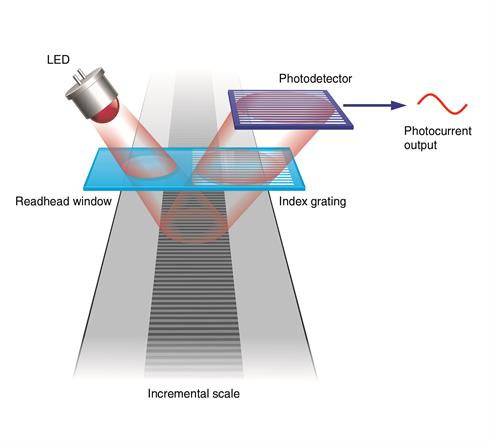
\includegraphics[width=0.7\linewidth]{./pics/sincos_encoder}
			\caption{SinCos Encoder Hardwareaufbau des Encoderkopfs mit Lineal. Das Index Grating ist nur eine transparente Platte.}
		\end{figure}
	\subsection{EnDat Encoder}
		Es gibt ein grobes Lineal in welchem die absolute Position kodiert ist und ein feineres für die inkrementalen Schritte (feinschritt). Die Digitalisierung des Positionswertes erfolgt oft direkt am Encoderkopf.
		\begin{figure}
			\centering
			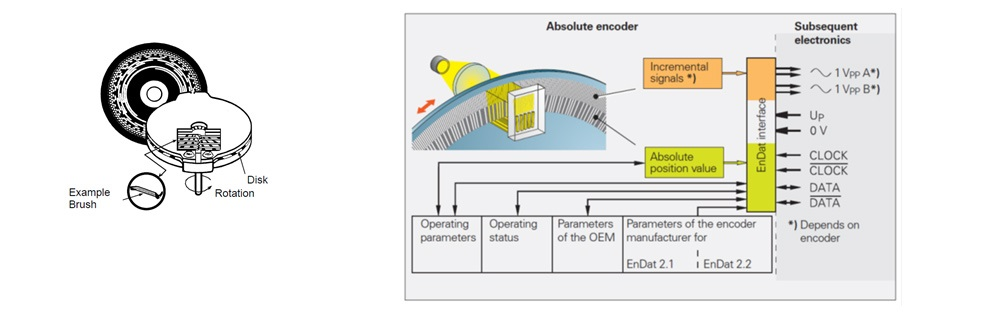
\includegraphics[width=\linewidth]{./pics/endat}
			\caption{Absolutencoder}
		\end{figure}
\section{Bussysteme}
	\subsection{EtherCAT}
		EtherCAT (Ethernet for Control Automation Technology) ist ein von der Firma \textbf{Beckhoff Automation} initiiertes Echtzeit-Ethernet.\\\\
		EtherCAT unterscheidet sich wesentlich von anderen Industrial Ethernet Lösungen. Während bei diesen der vom Master versendete Standard Ethernet Frame (gemäß IEEE 802.3) in jeder Anschaltung zunächst empfangen, dann interpretiert und die Prozessdaten weiterkopiert werden, entnehmen beim EtherCAT die EtherCAT Slave-Geräte die für sie bestimmten Daten, während das Telegramm das Gerät durchläuft. Ebenso werden Eingangsdaten im Durchlauf in das Telegramm eingefügt.\\\\
		Zykluszeiten $ \leq 100 \mu s $ mit niedrigem Jitter.
	\subsection{ETEL Systeme}
		\subsubsection{TransnET}
			Für Echtzeit-Anwendungen mit mehreren Achsen. Die TransnET Synchronisation mit Jitter im Nanosekunden-Bereich ist die richtige Lösung für deterministische und zuverlässige Kommunikation innerhalb von Maschinen.
		\subsubsection{Turbo-ETEL-Bus}
			Multi-axis fast bus mit 100Mbps
	\subsection{CAN-Bus}
		Der CAN-Bus (Controller Area Network) ist ein serielles Bussystem und gehört zu den Feldbussen. Feldbus ist ein Bussystem zur Kommunikation für Sensoren, Aktoren in einer Anlage bzw. Maschine.\\\\
		\textbf{Funktionsprinzip}: Der CAN-Bus arbeitet nach dem „Multi-Master-Prinzip“ d. h., er verbindet mehrere gleichberechtigte Steuergeräte. Ein CSMA/CR-Verfahren löst Kollisionen (gleichzeitiger Buszugriff) auf, ohne dass die gewinnende, höher priorisierte Nachricht beschädigt wird. Der CAN-Bus ist nicht echtzeitfähig, da nicht garantiert werden kann ob der Bus zu gegebenen Zeitpunkt gerade frei ist.
	\subsection{Ginlink}
		Busverbindung vom COPMAS zum Hammer.